\chapter{\inverseMatTitle}
\label{inverse_matrix}


\begin{definition}
A square matrix $M$ is \emph{invertible} (or \emph{nonsingular})\index{Invertible}\index{Nonsingular} if there exists a matrix $M^{-1}$ such that
\[
M^{-1}M=I=M^{-1}M.
\]
\end{definition}

%\begin{figure}
%\begin{center}
%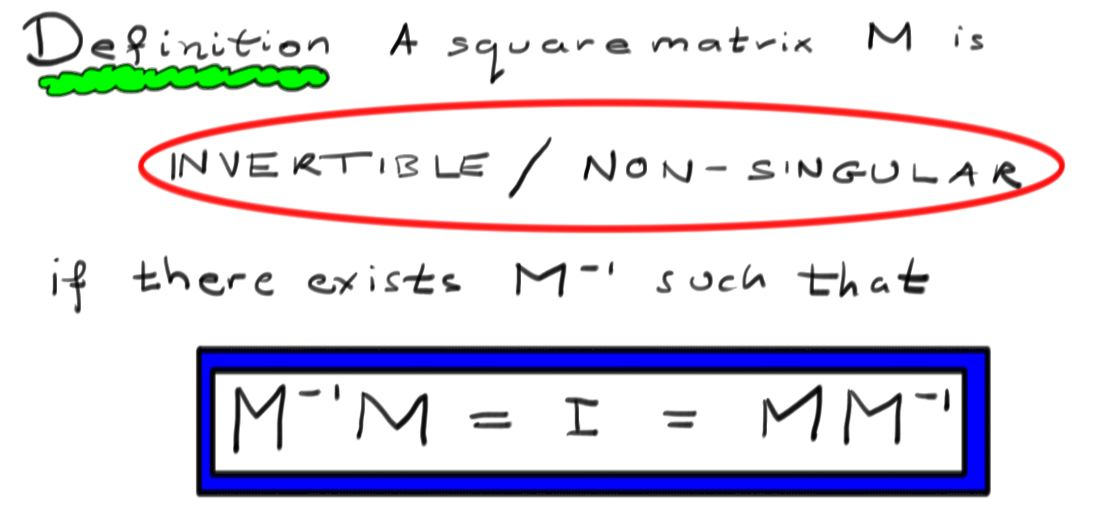
\includegraphics[scale=.27]{\inverseMatPath/defn_inverse_matrix.jpg}
%\end{center}
%\end{figure}


\begin{remark}[Inverse of a $2\times 2$ Matrix] Let $M$ and $N$ be the matrices:
\[
M=\begin{pmatrix}
a & b \\
c & d \\
\end{pmatrix},\qquad N=\begin{pmatrix}
d & -b \\
-c & a \\
\end{pmatrix}
\]
Multiplying these matrices gives:
\[
MN=\begin{pmatrix}
ad-bc & 0 \\
0 & ad-bc \\
\end{pmatrix}=(ad-bc)I
\]

Then $M^{-1}=\frac{1}{ad-bc}\begin{pmatrix}
d & -b \\
-c & a \\
\end{pmatrix}$, so long as $ad-bc\neq 0$.    
\end{remark}

\begin{figure}
\begin{center}
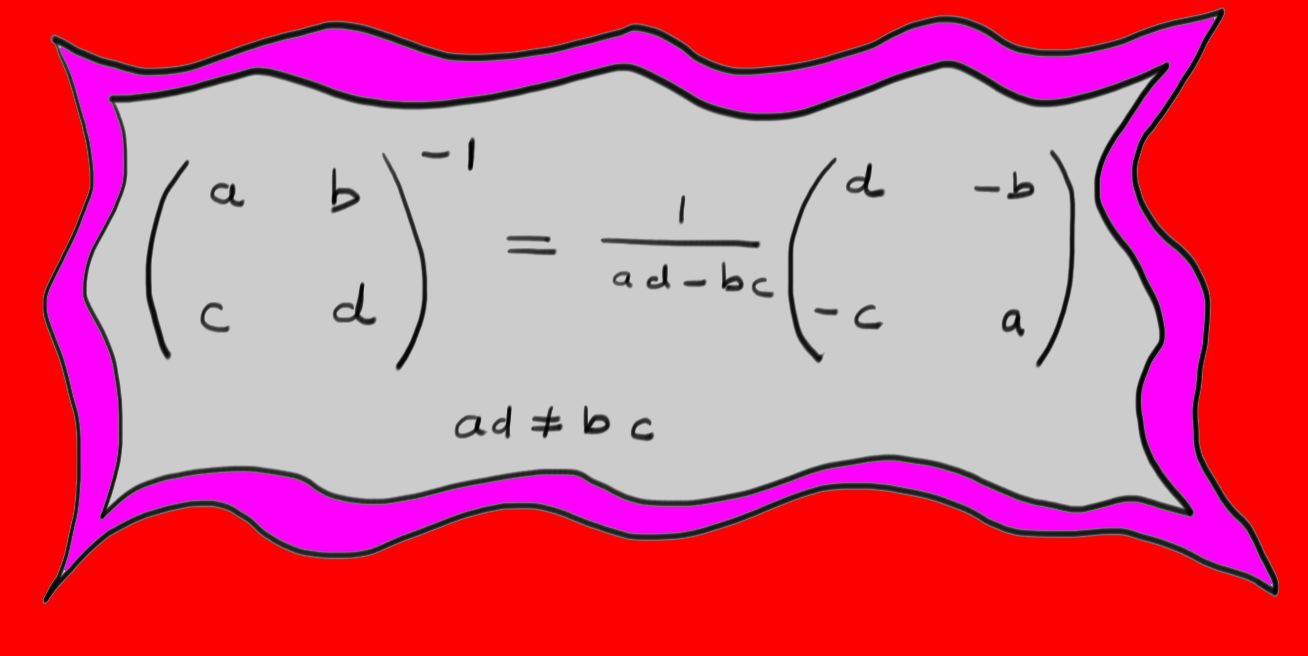
\includegraphics[scale=.24]{\inverseMatPath/2x2_inverse.jpg}
\end{center}
\caption{The formula for the inverse of a 2$\times$2 matrix is worth memorizing!}
\end{figure}



\section{Three Properties of the Inverse}

\begin{enumerate}
\item If $A$ is a square matrix and $B$ is the inverse of $A$, then $A$ is the inverse of $B$, since $AB=I=BA$.  Then we have the identity:
\[
(A^{-1})^{-1}=A
\]

\item Notice that $B^{-1}A^{-1}AB=B^{-1}IB=I=ABB^{-1}A^{-1}$.
Then:
\[
(AB)^{-1}=B^{-1}A^{-1}
\]
Then much like the transpose, taking the inverse of a product \emph{reverses} the order of the product.


\begin{center}
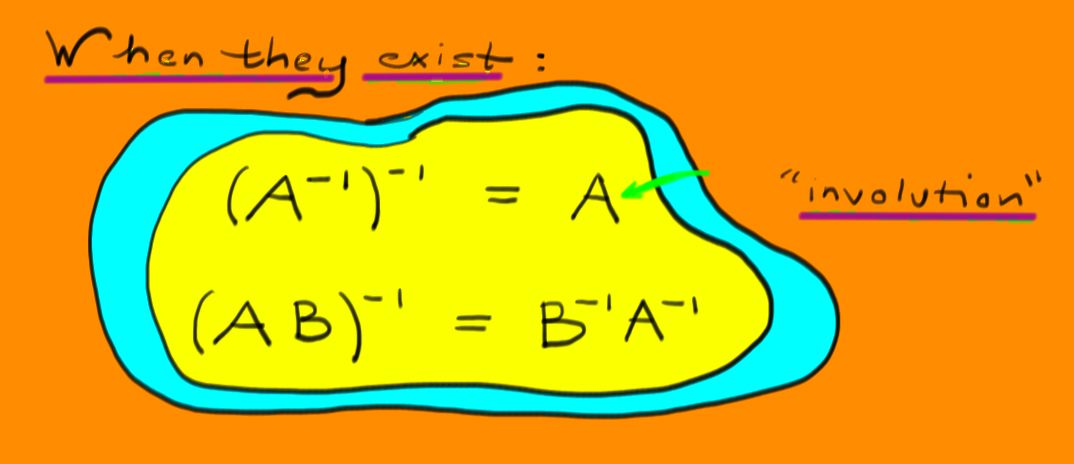
\includegraphics[scale=.26]{\inverseMatPath/inverse_inverse.jpg}
\end{center}

\item Finally, recall that $(AB)^T=B^TA^T$.  Since $I^T=I$, then $(A^{-1}A)^T=A^T(A^{-1})^T=I$.  Similarly, $(AA^{-1})^T=(A^{-1})^TA^T=I$.  Then:
\[
(A^{-1})^T=(A^T)^{-1}
\]
%As such, we could even write $A^{-T}$ for the inverse of the transpose of $A$ (or equivalently the transpose of the inverse).
\begin{center}
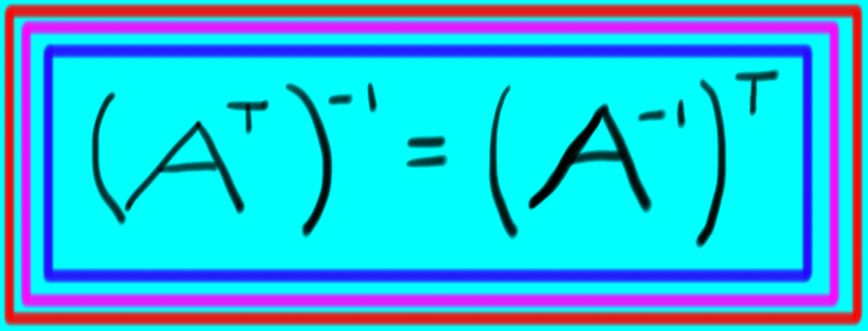
\includegraphics[scale=.20]{\inverseMatPath/transpose_inverse.jpg}
\end{center}
\end{enumerate}

\videoscriptlink{inverse_matrix_2by2_example.mp4}{Example}{scripts_inverse_matrix_2by2_example}




\section{Finding Inverses}

Suppose $M$ is a square matrix and $MX=V$ is a linear system with unique solution $X_0$.  Since there is a unique solution, $M^{-1}V$, then the reduced row echelon form of the linear system has an identity matrix on the left:
\[
\begin{amatrix}{1}
M & V
\end{amatrix}
\sim
\begin{amatrix}{1}
I & M^{-1}V
\end{amatrix}
\]
Solving the linear system $MX=V$ then tells us what $M^{-1}V$ is.  

To solve many linear systems with the same matrix at once, 
\[MX=V_1,~MX=V_2\]

we can consider augmented matrices with 
%a matrix on the right side instead of a column vector, 
many columns on the right 
 and then apply Gaussian row reduction to the left side of the matrix.  Once the identity matrix is on the left side of the augmented matrix, then the solution of each of the individual linear systems is on the right.
 \[
\left(\begin{array}{c|cc}
M & V_1&V_2
\end{array}\right)
\sim
\left(\begin{array}{c|cc}
I & M^{-1}V_1 & M^{-1}V_2
\end{array}\right)
\]


To compute $M^{-1}$, we would like $M^{-1}$, rather than $M^{-1}V$ to appear on the right side of our augmented matrix.
This is achieved by  solving the collection of systems $MX=e_k$, where $e_k$ is the column vector of zeroes with a $1$ in the $k$th entry.  
{\itshape I.e.,} the $n\times n$ identity matrix can be viewed as a bunch of column vectors $I_n=(e_1 \ e_2 \ \cdots e_n)$. So, putting the $e_k$'s together into an identity matrix, we get:
\[
\begin{amatrix}{1}
M & I
\end{amatrix}
\sim
\begin{amatrix}{1}
I & M^{-1}I
\end{amatrix}
=\begin{amatrix}{1}
I & M^{-1}
\end{amatrix}
\]


\begin{example}
Find $\begin{pmatrix}
-1 & 2 & -3 \\
2 & 1 & 0 \\
4 & -2 & 5 \\
\end{pmatrix}^{-1}
$.
Start by writing the augmented matrix, then apply row reduction to the left side.

\begin{align*}
\begin{pmat}{rrr|ccc}
-1 & 2 & -3 & 1 & 0 & 0 \\[1mm]
2  & 1 &  0 & 0 & 1 & 0 \\[1mm]
 4 & -2 & 5 & 0 & 0 & 1
\end{pmat} & \sim \begin{pmat}{crr|ccc}
1  & -2&  3  & 1 & 0 & 0 \\[1mm]
0  & 5 &  -6 & 2 & 1 & 0 \\[1mm]
 0 & 6 & -7  & 4 & 0 & 1
\end{pmat} \\[2mm]
& \sim \begin{pmat}{ccr|rrc}
1  & 0 &  \frac{3}{5}  & -\frac{1}{4} & \frac{2}{5} & 0 \\[1mm]
0  & 1 &  -\frac{6}{5} & \frac{2}{5} & \frac{1}{5}  & 0 \\[1mm]
 0 & 0 &  \frac{1}{5}  & \frac{4}{5} & -\frac{6}{5} & 1
\end{pmat} \\[2mm]
& \sim \begin{pmat}{ccc|rrr}
1  & 0 &  0  & -5 & 4 & -3 \\[1mm]
0  & 1 &  0  & 10 & -7 & 6 \\[1mm]
 0 & 0 &  1  & 8 & -6 & 5
\end{pmat}
\end{align*}
At this point, we know $M^{-1}$ assuming we didn't goof up\index{Goofing up}.  However, row reduction is a lengthy and arithmetically involved process, so we should~\emph{check our answer,} by confirming that $MM^{-1}=I$ (or if you prefer $M^{-1}M=I$):
\[MM^{-1} = 
\begin{pmatrix}
-1 & 2 & -3 \\
2 & 1 & 0 \\
4 & -2 & 5 \\
\end{pmatrix}\begin{pmatrix}
-5 & 4 & -3 \\
10 & -7 & 6 \\
 8 & -6 & 5 \\
\end{pmatrix}
=\begin{pmatrix}
1 & 0 & 0 \\
0 & 1 & 0 \\
0 & 0 & 1 \\
\end{pmatrix}
\]  
The product of the two matrices is indeed the identity matrix, so we're done.
\end{example}

%\href{\webworkurl ReadingHomework10/1/}{Reading homework: problem 10.1}
\reading{10}{1}
\section{Linear Systems and Inverses}

If $M^{-1}$ exists and is known, then we can immediately solve linear systems associated to $M$.

\begin{example}
Consider the linear system:
\[
      \begin{linsys}{2}
            -x & +2y & -3z         &=& 1  \\[1mm]
            2x & +\ y\,   &             &=& 2 \\[1mm]
            4x & -2y & +5z         &=& 0  
      \end{linsys}
\]
The associated matrix equation is $MX=\colvec{1\\2\\0},$ where \(M\) is the same as in the previous section.  Then:
\[
\colvec{x\\y\\z}=\begin{pmatrix}
-1 & 2 & -3 \\
2 & 1 & 0 \\
4 & -2 & 5 \\
\end{pmatrix}^{-1}\colvec{1\\2\\0}
=\begin{pmatrix}
-5 & 4 & -3 \\
10 & -7 & 6 \\
 8 & -6 & 5 \\
\end{pmatrix}\colvec{1\\2\\0}
=\colvec{3\\-4\\-4}
\]
Then $\colvec{x\\y\\z}=\colvec{3\\-4\\-4}$.  
In summary, when $M^{-1}$ exists, then \[MX=V \Rightarrow X=M^{-1}V\, .\]
\end{example}



%\href{\webworkurl ReadingHomework10/2/}{Reading homework: problem 10.2}
\reading{10}{2}

\section{Homogeneous Systems}

\begin{theorem}
A square matrix $M$ is invertible if and only if the homogeneous system \[MX=0\] has no non-zero solutions.
\end{theorem}

\begin{proof}
First, suppose that $M^{-1}$ exists.  Then $MX=0 \Rightarrow X=M^{-1}0=0$.  Thus, if $M$ is invertible, then $MX=0$ has no non-zero solutions.

On the other hand, $MX=0$ always has the solution $X=0$.  If no other solutions exist, then $M$ can be put into reduced row echelon form with every variable a pivot.  In this case, $M^{-1}$ can be computed using the process in the previous section.
\end{proof}

%\begin{figure}
\begin{center}
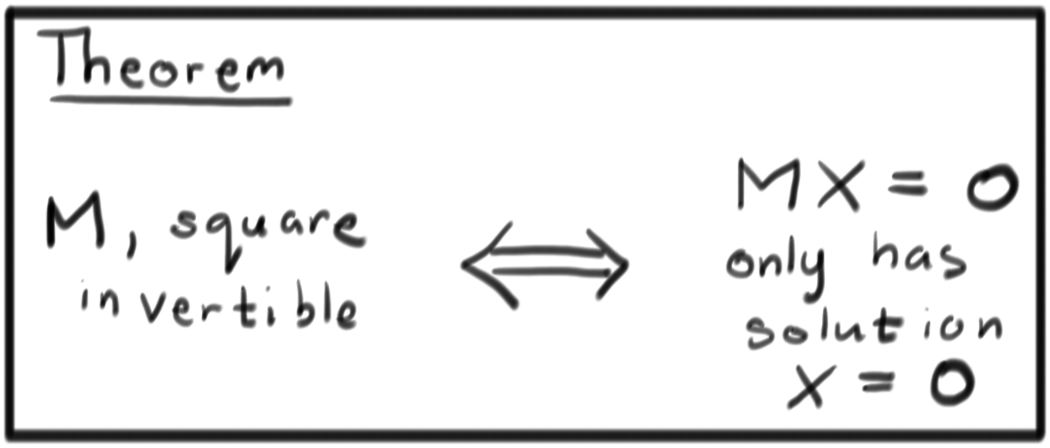
\includegraphics[scale=.26]{\inverseMatPath/inverse_theorem.jpg}
\end{center}
%\end{figure}

%A great test of your linear algebra knowledge is to make a list of conditions for a matrix to be singular.
%You will learn more of these as the course goes by, but can also skip straight to the list in Section~\ref{thelist}. 

\section{Bit Matrices}\index{Bit matrices}
In computer science, information is recorded using binary strings of data.  For example, the following string contains an English word:
\[
011011000110100101101110011001010110000101110010
\]
A \hypertarget{bits}{\emph{bit}} is the basic unit of information, keeping track of a single one or zero.  Computers can add and multiply individual bits very quickly.

Consider the set $\Z_2=\{0,1 \}$ with addition and multiplication given by the following tables:
\label{Z2}
\[
\begin{array}{c|cc}
+ & 0 & 1 \\ \hline
0 & 0 & 1 \\
1 & 1 & 0 \\
\end{array}
\qquad
\begin{array}{c|cc}
\cdot & 0 & 1 \\ \hline
0 & 0 & 0 \\
1 & 0 & 1 \\
\end{array}
\]
Notice that $-1=1$, since $1+1=0$.

It turns out that $\Z_2$ is almost as good as the real or complex numbers (they are all \hyperref[fields]{fields}), so we can apply all of the linear algebra we have learned thus far to matrices with $\Z_2$ entries.  A matrix with entries in $\Z_2$ is sometimes called a \emph{bit matrix}\footnote{Note that bits in a bit arithmetic shorthand do not ``add'' and ``multiply'' as elements in $\mathbb{Z}_2$ does since these operators corresponding to ``bitwise or'' and ``bitwise and'' respectively.}.

\begin{example}
$\begin{pmatrix}
1 & 0 & 1 \\
0 & 1 & 1 \\
1 & 1 & 1 \\
\end{pmatrix}$ is an invertible matrix over $\Z_2$:
\[\begin{pmatrix}
1 & 0 & 1 \\
0 & 1 & 1 \\
1 & 1 & 1 \\
\end{pmatrix}^{-1}=\begin{pmatrix}
0 & 1 & 1 \\
1 & 0 & 1 \\
1 & 1 & 1 \\
\end{pmatrix}
\]

This can be easily verified by multiplying:
\[\begin{pmatrix}
1 & 0 & 1 \\
0 & 1 & 1 \\
1 & 1 & 1 \\
\end{pmatrix}\begin{pmatrix}
0 & 1 & 1 \\
1 & 0 & 1 \\
1 & 1 & 1 \\
\end{pmatrix}=\begin{pmatrix}
1 & 0 & 0 \\
0 & 1 & 0 \\
0 & 0 & 1 \\
\end{pmatrix}
\]
\end{example}

\begin{remark}[Application: Cryptography]  
A very simple way to hide information is to use a substitution cipher, in which the alphabet is permuted and each letter in a message is systematically exchanged for another.  For example, the ROT-13 cypher just exchanges a letter with the letter thirteen places before or after it in the alphabet.  For example, HELLO becomes URYYB.  Applying the algorithm again decodes the message, turning URYYB back into HELLO.  Substitution ciphers are easy to break, but the basic idea can be extended to create cryptographic systems that are practically uncrackable.  For example, a \emph{one-time pad} is a system that uses a different substitution for each letter in the message.  So long as a particular set of substitutions is not used on more than one message, the one-time pad is unbreakable.

English characters are often stored in computers in the ASCII format.  In ASCII, a single character is represented by a string of eight bits, which we can consider as a vector in $\Z_2^8$ (which is like vectors in $\Re^8$, where the entries are zeros and ones).  One way to create a substitution cipher, then, is to choose an $8\times 8$ invertible bit matrix $M$, and multiply each letter of the message by $M$.  Then to decode the message, each string of eight characters would be multiplied by $M^{-1}$.  

To make the message a bit tougher to decode, one could consider pairs (or longer sequences) of letters as a single vector in $\Z_2^{16}$ (or a higher-dimensional space), and then use an appropriately-sized invertible matrix.

For more on cryptography, see ``The Code Book,'' by Simon Singh (1999, Doubleday).
\end{remark}

%{\itshape You should now be ready to attempt the \hyperref[sample1]{first sample midterm}.}
%\begin{center}
%\shabox{
%\begin{tabular}{c}
%\itshape \hyperref[sample1]{You are now ready to attempt the first sample midterm}. 
%\\
%\hyperref[sample1]{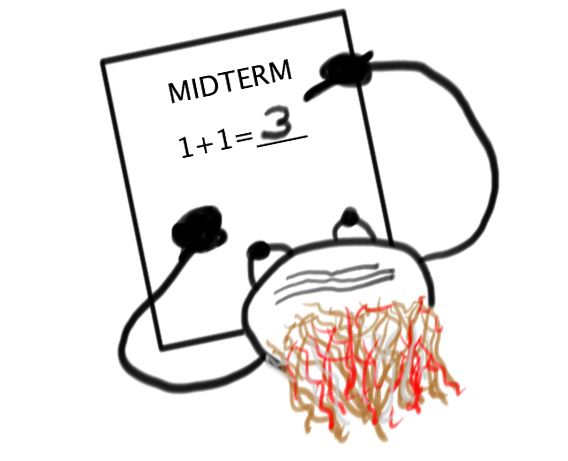
\includegraphics[scale=.15]{midterm.jpg}}
%\end{tabular}
%}
%\end{center}
%
%\section*{References}
%
%Hefferon: Chapter Three, Section IV.2
%\\
%Beezer: Chapter M, Section MISLE
%\\
%Wikipedia:
%\href{http://en.wikipedia.org/wiki/Invertible_matrix}{Invertible Matrix}
%
%
\section{Review Problems}




\begin{enumerate}
\item \label{det33} Let $M=\begin{pmatrix}
m^1_1 & m^1_2 & m^1_3\\
m^2_1 & m^2_2 & m^2_3\\
m^3_1 & m^3_2 & m^3_3\\
\end{pmatrix}$.  Use row operations to put $M$ into \emph{row echelon form}.  For simplicity, assume that $m_1^1\neq 0 \neq m^1_1m^2_2-m^2_1m^1_2$.

Prove that $M$ is non-singular if and only if:
\[
m^1_1m^2_2m^3_3 
- m^1_1m^2_3m^3_2 
+ m^1_2m^2_3m^3_1 
- m^1_2m^2_1m^3_3 
+ m^1_3m^2_1m^3_2
- m^1_3m^2_2m^3_1
\neq 0
\]

\phantomnewpage

\item 
\begin{enumerate}
\item What does the matrix $E^1_2=\begin{pmatrix}
0 & 1 \\
1 & 0
\end{pmatrix}$ do to $M=\begin{pmatrix}
a & b \\
d & c
\end{pmatrix}$ under left multiplication?  What about right multiplication?
\item Find elementary matrices $R^1(\lambda)$ and $R^2(\lambda)$ that respectively multiply rows $1$ and $2$ of $M$ by $\lambda$ but otherwise leave $M$ the same under left multiplication.
\item Find a matrix $S^1_2(\lambda)$ that adds a multiple $\lambda$ of row $2$ to row $1$ under left multiplication.
\end{enumerate}

\phantomnewpage

\item Let $M$ be a matrix and $S^i_jM$ the same matrix with rows \(i\) and \(j\) switched.  Explain every line of the 
\hyperlink{rowswap}{series of equations} proving that $\det M = -\det (S^i_jM)$.

\phantomnewpage

%\item \label{prob_inversion_number} This problem is a ``hands-on'' look at why \hyperlink{permutation_parity}{the property} describing the parity of permutations is true.
%
%\hypertarget{inversion_number}{The \emph{inversion number}}\index{Permutation!Inversion number} of a permutation $\sigma$ is the number of pairs $i<j$ such that $\sigma(i)>\sigma(j)$; it's the number of ``numbers that appear left of smaller numbers'' in the permutation.  For example, for the permutation $\rho = [4,2,3,1]$, the inversion number is $5$. The number $4$ comes before $2,3,$ and $1$, and $2$ and $3$ both come before $1$.
%
%Given a permutation $\sigma$, we can make a new permutation $\tau_{i,j} \sigma$ by exchanging the $i$th and $j$th entries of $\sigma$.
%
%\begin{enumerate}
%\item What is the inversion number of the permutation \(\mu=[1,2,4,3]\) that exchanges 4 and 3 and leaves everything else alone? Is it an even or an odd permutation?
%
%\item What is the inversion number of the permutation \(\rho=[4,2,3,1]\) that exchanges 1 and 4 and leaves everything else alone? Is it an even or an odd permutation?
%
%\item What is the inversion number of the permutation \(\tau_{1,3} \mu\)? Compare the parity\footnote{The \emph{parity} of an integer refers to whether the integer is even or odd. Here the parity of a permutation $\mu$ refers to the parity of its inversion number.} of \(\mu\) to the parity of \(\tau_{1,3} \mu.\)
%
%\item What is the inversion number of the permutation \(\tau_{2,4} \rho\)? Compare the parity of \(\rho\) to the parity of \(\tau_{2,4} \rho.\)
%
%\item What is the inversion number of the permutation \(\tau_{3,4} \rho\)? Compare the parity of \(\rho\) to the parity of \(\tau_{3,4} \rho.\)
%\end{enumerate}
%
%\videoscriptlink{elementary_matrices_determinant_hint.mp4}{Problem~\ref{prob_inversion_number} hints}{scripts_elementary_matrices_determinants_hint}

\phantomnewpage

%\item \label{problem_permutation} (Extra credit) Here we will examine a (very) small set of the general properties about permutations and their applications. In particular, we will show that one way to compute the sign of a permutation is by finding the \hyperlink{inversion_number}{inversion number} $N$ of $\sigma$ and we have
%\[
%\sgn(\sigma) = (-1)^N.
%\]
%
%For this problem, let $\mu = [1,2,4,3]$.
%
%\begin{enumerate}
%\item Show that every permutation $\sigma$ can be sorted by only taking simple (adjacent) transpositions\index{Permutation!Simple transposition} $s_i$ where $s_i$ interchanges the numbers in position $i$ and $i+1$ of a permutation $\sigma$ (in our other notation $s_i = \tau_{i,i+1}$). For example $s_2 \mu = [1, 4, 2, 3]$, and to sort $\mu$ we have $s_3 \mu = [1, 2, 3, 4]$.
%
%\item \label{prob_part_relations} We can compose simple transpositions together to represent a permutation (note that the sequence of compositions is not unique), and these are associative, we have an identity (the trivial permutation where the list is in order or we do nothing on our list), and we have an inverse since it is clear that $s_i s_i \sigma = \sigma$. Thus permutations of $[n]$ under composition are an example of a \hyperref[groups]{group}. However note that not all simple transpositions commute with each other since
%\begin{align*}
%s_1 s_2 [1, 2, 3] & = s_1 [1, 3, 2] = [3, 1, 2]
%\\ s_2 s_1 [1, 2, 3] & = s_2 [2, 1, 3] = [2, 3, 1]
%\end{align*}
%(you will prove here when simple transpositions commute). When we consider our initial permutation to be the trivial permutation $e = [1, 2, \dotsc, n]$, we do not write it; for example $s_i \equiv s_i e$ and $\mu = s_3 \equiv s_3 e$. This is analogous to not writing 1 when multiplying. Show that $s_i s_i = e$ (in shorthand $s_i^2 = e$), $s_{i+1} s_i s_{i+1} = s_i s_{i+1} s_i$ for all $i$, and $s_i$ and $s_j$ commute for all $|i - j| \geq 2$.
%
%\item Show that every way of expressing $\sigma$ can be obtained from using the relations proved in part~\ref{prob_part_relations}. In other words, show that for any expression $w$ of simple transpositions representing the trivial permutation $e$, using the proved relations.
%
%\emph{Hint: Use induction on $n$. For the induction step, follow the path of the $(n+1)$-th strand by looking at $s_n s_{n-1} \cdots s_k s_{k\pm1} \cdots s_n$ and argue why you can write this as a subexpression for any expression of $e$. Consider using diagrams of these paths to help.}
%
%\item The simple transpositions \hyperlink{action}{acts on} an $n$-dimensional vector space $V$ by $s_i v = E^i_{i+1} v$ (where $E^i_j$ is \hyperlink{elem_matrix_row_swap}{an elementary matrix}) for all vectors $v \in V$. Therefore we can just represent a permutation $\sigma$ as the matrix $M_{\sigma}$\footnote{Often people will just use $\sigma$ for the matrix when the context is clear.}, and we have $\det(M_{s_i}) = \det(E^i_{i+1}) = -1$. Thus prove that $\det(M_{\sigma}) = (-1)^N$ where $N$ is a number of simple transpositions needed to represent $\sigma$ as a permutation. You can assume that $M_{s_i s_j} = M_{s_i} M_{s_j}$ (it is not hard to prove) and that $\det(A B) = \det(A) \det(B)$ \hyperref[detmultiplicative]{from Chapter~\ref*{elementarydeterminantsII}}.
%
%\emph{Hint: You to make sure $\det(M_{\sigma})$ is well-defined since there are infinite ways to represent $\sigma$ as simple transpositions.}
%
%\item Show that $s_{i+1} s_i s_{i+1} = \tau_{i, i+2}$, and so give one way of writing $\tau_{i, j}$ in terms of simple transpositions? Is $\tau_{i,j}$ an even or an odd permutation? What is $\det(M_{\tau_{i,j}})$? What is the inversion number of $\tau_{i,j}$?
%
%\item The minimal number of simple transpositions needed to express $\sigma$ is called the \emph{length}\index{Permutation!Length} of $\sigma$; for example the length of $\mu$ is 1 since $\mu = s_3$. Show that the length of $\sigma$ is equal to the inversion number of $\sigma$.
%
%\emph{Hint: Find an procedure which gives you a new permutation $\sigma^{\prime}$ where $\sigma = s_i \sigma^{\prime}$ for some $i$ and the inversion number for $\sigma^{\prime}$ is 1 less than the inversion number for $\sigma$.}
%
%\item Show that $(-1)^N = \sgn(\sigma) = \det(M_{\sigma})$, where $\sigma$ is a permutation with $N$ inversions. Note that this immediately implies that $\sgn(\sigma \rho) = \sgn(\sigma) \sgn(\rho)$ for any permutations $\sigma$ and $\rho$.
%\end{enumerate}

\item Let $M'$ be the matrix obtained from $M$ by swapping two columns $i$ and $j$. Show that $\det M'=-\det M $.

\item The scalar triple product of three vectors $u,v,w$ from $\Re^3$ is $u\cdot(v\times w)$. Show that this product is the same as the determinant of the matrix whose columns are $u,v,w$ (in that order). What happens to the scalar triple product when the factors are permuted? 

\item Show that if $M$ is a $3\times 3$ matrix whose third row is a sum of multiples of the other rows ($R_3=aR_2+bR_1$) then $\det M=0$. Show that the same is true if one of the columns is a sum of multiples of the others. 

\end{enumerate}

\phantomnewpage

\newpage


